% =====================================================================
\newpage
\section{Математическое описание}
\label{sec:math}

\subsection{Конечный автомат}

Конечным автоматом Мура называется набор
\[
	M = (Q, X, Y, \delta, \lambda, q_0),
\]
где
\begin{itemize}
	\item $Q$ --- конечное множество состояний;
	\item $X$ --- конечный входной алфавит;
	\item $Y$ --- конечный выходной алфавит;
	\item $\delta: Q \times X \to Q$ --- функция переходов;
	\item $\lambda: Q \to Y$ --- функция выходов;
	\item $q_0 \in Q$ --- начальное состояние.
\end{itemize}

% Автомат работает в дискретном времени $t = 0, 1, 2, \dots$: в каждый такт он выдает выходной символ $y(t)$, зависящий только от текущего состояния $q(t)$, и по входному символу $x(t) \in X$ переходит в состояние $q(t+1)$:
% \[
% 	y(t) = \lambda\bigl(q(t)\bigr), \qquad q(t+1) = \delta\bigl(q(t),\ x(t)\bigr), \qquad q(0) = q_0.
% \]
% Функцию переходов конечного автомата можно задать таблицей размером $|Q| \times |X|$.

% Пятерку $(Q, X, Y, \delta, \lambda)$ без начального состояния называют неинициальным автоматом; выбор $q_0 \in Q$ превращает его в инициальный автомат.

\subsection{Клеточный автомат}
\label{sec:ca}

Клеточный автомат --- это совокупность одинаковых конечных автоматов (клеток), расположенных в узлах регулярной решетки и соединенных между собой так, что входной символ каждого автомата образуют выходные символы его соседей. Все автоматы работают синхронно, по общим тактам времени~\cite{tema, neumann}.

Формально клеточный автомат задается тройкой
\[
	A = (L, \mathcal{N}, M),
\]
где
\begin{itemize}
	\item $L = \mathbb{Z}_n \times \mathbb{Z}_n = \{(i, j) : i, j \in \{0, 1, \dots, n-1\}\}$ --- решетка клеток: квадратное поле $n \times n$ с тороидальными граничными условиями, $i$ --- номер строки, $j$ --- номер столбца;
	\item $\mathcal{N} = \bigl((-1, 0),\ (0, 1),\ (0, -1),\ (1, 0)\bigr)$ --- окрестность фон Неймана: сдвиги к соседям $N$, $E$, $W$, $S$; вход клетки $(i, j)$ соединен с выходами клеток $(i, j) + v$, $v \in \mathcal{N}$;
	\item $M = (Q, X, Y, \delta, \lambda)$ --- автомат Мура клетки без фиксированного начального состояния: $Q = Y = \{0, 1\}$ (0 --- «мертвая», 1 --- «живая»), $\lambda(q) = q$, $X = Q^4$, $\delta\bigl(C, (N, E, W, S)\bigr) = f(C, N, E, W, S)$, где $f: Q^5 \to Q$ задается номером правила.
\end{itemize}

Отображение $\sigma^t: L \to Q$, сопоставляющее каждой клетке ее состояние в момент $t$, называется конфигурацией. Начальная конфигурация $\sigma^0$ задается пользователем: клетка $(i, j)$, $0 \le i, j \le n-1$, --- это автомат $M$ с начальным состоянием $q_0 = \sigma^0(i, j)$.

% В данной работе:
% \begin{itemize}
% 	\item $Q = \{0, 1\}$ --- состояния клетки: 0 --- «мертвая», 1 --- «живая»;
% 	\item $Y = Q$, $\lambda(q) = q$ --- клетка передает соседям свое состояние;
% 	\item $\mathcal{N} = \bigl((-1, 0),\ (0, 1),\ (0, -1),\ (1, 0)\bigr)$ --- четыре соседа окрестности фон Неймана в порядке «север, восток, запад, юг» (раздел~\ref{sec:neumann}). Сама клетка $C$ в $\mathcal{N}$ не включается: ее состояние учитывается как первый аргумент функции $\delta$;
% 	\item $X = Q^4$ --- входной символ клетки $(i, j)$ есть набор состояний ее соседей:
% 	\[
% 		x_{i,j}(t) = \bigl(q_{i-1,j}(t),\ q_{i,j+1}(t),\ q_{i,j-1}(t),\ q_{i+1,j}(t)\bigr) = (N, E, W, S),
% 	\]
% 	поэтому входной алфавит содержит $|X| = 2^4 = 16$ символов;
% 	\item $\delta: Q \times X \to Q$ --- функция переходов; ее таблица содержит $|Q| \cdot |X| = 2 \cdot 16 = 32$ значения и задается номером правила (раздел~\ref{sec:rule}). Функцию переходов удобно записывать как функцию пяти переменных --- состояния клетки и состояний четырех соседей:
% 	\[
% 		\delta\bigl(C, (N, E, W, S)\bigr) = f(C, N, E, W, S), \qquad f: Q^5 \to Q;
% 	\]
% 	\item $\sigma^0$ задается пользователем вручную или случайным образом.
% \end{itemize}

% Таким образом, каждая клетка $(i, j)$ --- это один и тот же автомат $M$, запущенный из своего начального состояния $q_{i,j}(0) = \sigma^0(i, j)$; клетки различаются только начальными состояниями. Работа клеточного автомата описывается системой
% \[
% 	q_{i,j}(t+1) = \delta\bigl(q_{i,j}(t),\ x_{i,j}(t)\bigr), \qquad (i, j) \in L,
% \]
% где все $n^2$ автоматов срабатывают одновременно. Поскольку выход автомата Мура зависит только от его состояния, входы всех клеток в момент $t$ однозначно определяются состояниями в момент $t$, и такая синхронная схема корректна.

% \begin{figure}[H]
% 	\centering
% 	\begin{tikzpicture}[>=stealth, thick]
% 		\node[draw, rounded corners, minimum width=3.4cm, minimum height=1.6cm, align=center] (m)
% 			{автомат клетки $(i, j)$\\ состояние $q_{i,j}(t)$};
% 		\node (n) at (0, 2.1) {$N = q_{i-1,j}$};
% 		\node (s) at (0, -2.1) {$S = q_{i+1,j}$};
% 		\node (w) at (-4.4, 0) {$W = q_{i,j-1}$};
% 		\node (e) at (4.4, 0) {$E = q_{i,j+1}$};
% 		\draw[->] (n) -- (m);
% 		\draw[->] (s) -- (m);
% 		\draw[->] (w) -- (m);
% 		\draw[->] (e) -- (m);
% 		\draw[->] (m.north east) -- node[above, sloped, font=\small] {выход $y = q_{i,j}$} (3.8, 1.9);
% 	\end{tikzpicture}
% 	\caption{Клетка как конечный автомат: вход --- состояния четырех соседей, выход --- собственное состояние}
% 	\label{fig:cell-fsm}
% \end{figure}

% Отображение $\sigma^t: L \to Q$, $\sigma^t(i, j) = q_{i,j}(t)$, называется конфигурацией (поколением) в момент $t$. Весь клеточный автомат на поле $n \times n$ также можно рассматривать как один конечный автомат без входа (автономный), состояниями которого являются конфигурации: множество $Q^L$ конечно и содержит $|Q|^{n^2} = 2^{n^2}$ элементов, а глобальная функция переходов $F: Q^L \to Q^L$ задается формулой
% \[
% 	F(\sigma)(i, j) = f\bigl(\sigma(i, j),\ \sigma(i-1, j),\ \sigma(i, j+1),\ \sigma(i, j-1),\ \sigma(i+1, j)\bigr), \qquad \sigma^{t+1} = F(\sigma^t).
% \]
% Из конечности множества состояний следует, что последовательность конфигураций в конечном счете становится периодической (раздел~\ref{sec:period}).

\subsection{Окрестность фон Неймана}
\label{sec:neumann}

Окрестность фон Неймана клетки $(i, j)$, $i, j \in \{0, \dots, n-1\}$, образуют сама клетка $C$ и четыре клетки, имеющие с ней общую сторону: северная $N$, восточная $E$, южная $S$ и западная $W$ (рис.~\ref{fig:neighborhood}):
\[
	C = (i, j), \quad N = (i-1, j), \quad E = (i, j+1), \quad S = (i+1, j), \quad W = (i, j-1),
\]
где индексы берутся по модулю $n$. Строки нумеруются сверху вниз, поэтому северный сосед находится в строке с меньшим номером.

Четыре соседа $N$, $E$, $W$, $S$ образуют вход автомата клетки, а сама клетка $C$ участвует в переходе через собственное состояние. Далее буквами $C$, $N$, $E$, $W$, $S$ обозначаются также состояния этих клеток в момент $t$, например $C = \sigma^t(i, j)$, $N = \sigma^t(i-1, j)$.

\begin{figure}[H]
	\centering
	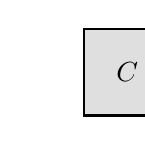
\begin{tikzpicture}[scale=1.1]
		\nbcell{1}{2}{$N$}
		\nbcell{0}{1}{$W$}
		\draw[thick, fill=gray!25] (1,1) rectangle ++(1,1); \node at (1.5,1.5) {$C$};
		\nbcell{2}{1}{$E$}
		\nbcell{1}{0}{$S$}
	\end{tikzpicture}
	\caption{Окрестность фон Неймана}
	\label{fig:neighborhood}
\end{figure}

\subsection{Функция перехода и номер правила}
\label{sec:rule}

Окрестность состоит из 5 клеток, каждая из которых имеет 2 состояния, поэтому существует $2^5 = 32$ различных набора $(C, N, E, W, S)$. Функция перехода $f: Q^5 \to Q$ сопоставляет каждому набору новое состояние центральной клетки:
\[
	\sigma^{t+1}(i, j) = f(C, N, E, W, S),
\]
то есть полностью задается 32 значениями. Всего существует $2^{32} \approx 4{,}3 \cdot 10^9$ таких функций. Для всех клеток $(i, j)$, $0 \le i, j \le n-1$, и всех моментов $t \ge 0$ в общем виде:
\[
	\sigma^{t+1}(i, j) = f\bigl(\sigma^t(i, j),\ \sigma^t(i-1, j),\ \sigma^t(i, j+1),\ \sigma^t(i, j-1),\ \sigma^t(i+1, j)\bigr),
\]
где индексы берутся по модулю $n$.

Пронумеруем наборы числами $idx \in \{0, \dots, 31\}$, двоичная запись которых есть $C\,N\,E\,W\,S$:
\[
	idx = 16C + 8N + 4E + 2W + S.
\]
Номер правила --- это число, разряд номер $idx$ двоичной записи которого равен значению $f$ на наборе с номером $idx$:
\[
	\text{№} = \sum_{idx=0}^{31} f(C, N, E, W, S) \cdot 2^{idx},
\]
откуда
\[
	f(C, N, E, W, S) = \left\lfloor \frac{\text{№}}{2^{idx}} \right\rfloor \bmod 2 = \left\lfloor \frac{\text{№}}{2^{16C + 8N + 4E + 2W + S}} \right\rfloor \bmod 2.
\]
Подставляя состояния клеток окрестности, получаем общую формулу перехода:
\[
	\sigma^{t+1}(i, j) = \left\lfloor \frac{\text{№}}{2^{\,16\sigma^t(i, j) + 8\sigma^t(i-1, j) + 4\sigma^t(i, j+1) + 2\sigma^t(i, j-1) + \sigma^t(i+1, j)}} \right\rfloor \bmod 2.
\]

Номер правила в двоичной системе счисления (дополнен незначащими нулями до 32 разрядов):
\[
	20\,874\,436_{10} = 0000\,0001\,0011\,1110\,1000\,0100\,1100\,0100_2.
\]
Таблица истинности функции $f$ приведена в таблице~\ref{tab:truth}.

\begin{table}[H]
	\centering
	\caption{Таблица истинности функции перехода (правило 20\,874\,436, порядок $C\,N\,E\,W\,S$)}
	\label{tab:truth}
	\small
	\begin{tabular}{|c|ccccc|c|}
		\hline
		$idx$ & $C$ & $N$ & $E$ & $W$ & $S$ & $f$ \\
		\hline
		0 & 0 & 0 & 0 & 0 & 0 & 0 \\
		1 & 0 & 0 & 0 & 0 & 1 & 0 \\
		2 & 0 & 0 & 0 & 1 & 0 & 1 \\
		3 & 0 & 0 & 0 & 1 & 1 & 0 \\
		4 & 0 & 0 & 1 & 0 & 0 & 0 \\
		5 & 0 & 0 & 1 & 0 & 1 & 0 \\
		6 & 0 & 0 & 1 & 1 & 0 & 1 \\
		7 & 0 & 0 & 1 & 1 & 1 & 1 \\
		8 & 0 & 1 & 0 & 0 & 0 & 0 \\
		9 & 0 & 1 & 0 & 0 & 1 & 0 \\
		10 & 0 & 1 & 0 & 1 & 0 & 1 \\
		11 & 0 & 1 & 0 & 1 & 1 & 0 \\
		12 & 0 & 1 & 1 & 0 & 0 & 0 \\
		13 & 0 & 1 & 1 & 0 & 1 & 0 \\
		14 & 0 & 1 & 1 & 1 & 0 & 0 \\
		15 & 0 & 1 & 1 & 1 & 1 & 1 \\
		\hline
	\end{tabular}
	\hspace{1cm}
	\begin{tabular}{|c|ccccc|c|}
		\hline
		$idx$ & $C$ & $N$ & $E$ & $W$ & $S$ & $f$ \\
		\hline
		16 & 1 & 0 & 0 & 0 & 0 & 0 \\
		17 & 1 & 0 & 0 & 0 & 1 & 1 \\
		18 & 1 & 0 & 0 & 1 & 0 & 1 \\
		19 & 1 & 0 & 0 & 1 & 1 & 1 \\
		20 & 1 & 0 & 1 & 0 & 0 & 1 \\
		21 & 1 & 0 & 1 & 0 & 1 & 1 \\
		22 & 1 & 0 & 1 & 1 & 0 & 0 \\
		23 & 1 & 0 & 1 & 1 & 1 & 0 \\
		24 & 1 & 1 & 0 & 0 & 0 & 1 \\
		25 & 1 & 1 & 0 & 0 & 1 & 0 \\
		26 & 1 & 1 & 0 & 1 & 0 & 0 \\
		27 & 1 & 1 & 0 & 1 & 1 & 0 \\
		28 & 1 & 1 & 1 & 0 & 0 & 0 \\
		29 & 1 & 1 & 1 & 0 & 1 & 0 \\
		30 & 1 & 1 & 1 & 1 & 0 & 0 \\
		31 & 1 & 1 & 1 & 1 & 1 & 0 \\
		\hline
	\end{tabular}
\end{table}

По таблице видно, что
\begin{itemize}
	\item живая клетка выживает при 6 конфигурациях соседей из 16, мертвая рождается при 5 из 16;
	\item пустая окрестность остается пустой ($idx = 0 \to 0$), а клетка, у которой живы все 5 клеток окрестности, умирает ($idx = 31 \to 0$);
	\item новое состояние зависит не только от состояния клетки и количества живых соседей, но и от того, какие именно соседи живы. Например, мертвая клетка с одним живым западным соседом рождается ($idx = 2 \to 1$), а с одним живым восточным --- нет ($idx = 4 \to 0$).
\end{itemize}

\subsection{Граничные условия}
\label{sec:torus}

В работе используются тороидальные граничные условия: противоположные края поля считаются соседними. Правый край поля склеивается с левым, а верхний --- с нижним, и поле превращается в поверхность тора, у которой нет границ. Все клетки при этом оказываются равноправными: окрестность любой клетки устроена одинаково.

Формально индексы клеток являются элементами $\mathbb{Z}_n$, а сложение индексов выполняется по модулю $n$. Для клетки $(i, j)$ с $i, j \in \{0, \dots, n-1\}$ соседи:
\begin{align*}
	N &= \bigl((i-1) \bmod n,\ j\bigr), & E &= \bigl(i,\ (j+1) \bmod n\bigr),\\
	S &= \bigl((i+1) \bmod n,\ j\bigr), & W &= \bigl(i,\ (j-1) \bmod n\bigr),
\end{align*}
где $i \bmod n \in \{0, \dots, n-1\}$ --- остаток от деления $i$ на $n$ (для $j$ --- так же); в частности, при $i = 0$ получаем $(i-1) \bmod n = n-1$, а при $i = n-1$ получаем $(i+1) \bmod n = 0$. То же верно для $j$: $(j-1) \bmod n = n-1$ при $j = 0$ и $(j+1) \bmod n = 0$ при $j = n-1$.

Для внутренних клеток ($0 < i < n-1$, $0 < j < n-1$) приведение по модулю ничего не меняет: $N = (i-1, j)$, $S = (i+1, j)$, $W = (i, j-1)$, $E = (i, j+1)$. Для клеток на краях поля один сосед берется с противоположного края:
\begin{itemize}
	\item верхняя строка ($i = 0$): северный сосед --- клетка $(n-1, j)$;
	\item нижняя строка ($i = n-1$): южный сосед --- клетка $(0, j)$;
	\item левый столбец ($j = 0$): западный сосед --- клетка $(i, n-1)$;
	\item правый столбец ($j = n-1$): восточный сосед --- клетка $(i, 0)$.
\end{itemize}

Угловая клетка лежит сразу на двух краях, поэтому с противоположных краев берутся два ее соседа: один по вертикали и один по горизонтали (таблица~\ref{tab:corners}).

\begin{table}[H]
	\centering
	\caption{Соседи угловых клеток на торе}
	\label{tab:corners}
	\begin{tabular}{|c|c|c|c|c|}
		\hline
		Клетка & $N$ & $E$ & $W$ & $S$ \\
		\hline
		$(0, 0)$         & $(n-1, 0)$   & $(0, 1)$     & $(0, n-1)$   & $(1, 0)$ \\
		$(0, n-1)$       & $(n-1, n-1)$ & $(0, 0)$     & $(0, n-2)$   & $(1, n-1)$ \\
		$(n-1, 0)$       & $(n-2, 0)$   & $(n-1, 1)$   & $(n-1, n-1)$ & $(0, 0)$ \\
		$(n-1, n-1)$     & $(n-2, n-1)$ & $(n-1, 0)$   & $(n-1, n-2)$ & $(0, n-1)$ \\
		\hline
	\end{tabular}
\end{table}

На торе четыре угловые клетки поля образуют квадрат $2 \times 2$: каждая из них соседствует с двумя другими угловыми клетками, а с противоположной по диагонали --- нет, так как диагональные клетки в окрестность фон Неймана не входят.

Далее считается, что $n \ge 3$: тогда все четыре соседа любой клетки различны и отличны от нее самой. При $n = 2$ северный и южный соседи совпадали бы, так как $(i-1) \bmod 2 = (i+1) \bmod 2$.

\subsection{Синхронное обновление}

Все клетки автомата обновляются одновременно: новое состояние каждой клетки вычисляется только по конфигурации $\sigma^t$:
\[
	\sigma^{t+1}(i, j) = f\bigl(\sigma^t(i, j),\ \sigma^t(i-1, j),\ \sigma^t(i, j+1),\ \sigma^t(i, j-1),\ \sigma^t(i+1, j)\bigr), \qquad 0 \le i, j \le n-1.
\]
Если записывать новые значения в то же поле, из которого читаются соседи, то часть клеток увидит соседей уже из поколения $t+1$, и результат будет зависеть от порядка обхода поля. Поэтому для вычисления шага используются два поля: из одного читается поколение $t$, в другое записывается поколение $t+1$.

\subsection{Сходимость и периодичность}
\label{sec:period}

Поле $n \times n$ с двумя состояниями клетки имеет конечное число конфигураций --- $2^{n^2}$. Автомат детерминирован: из одной конфигурации всегда получается одна и та же. Поэтому не более чем через $2^{n^2}$ шагов некоторая конфигурация обязательно повторится, и начиная с этого момента эволюция становится периодической:
\[
	\sigma^0 \to \sigma^1 \to \dots \to \sigma^{t_0} \to \dots \to \sigma^{t_0 + p - 1} \to \sigma^{t_0 + p} = \sigma^{t_0}.
\]
Здесь $t_0$ --- предпериод (длина переходного процесса), $p$ --- период. Если $p = 1$, конфигурация больше не меняется --- это неподвижная точка. Если $\sigma^{t_2} = \sigma^{t_1}$ для некоторых $t_1 < t_2$ и все предыдущие конфигурации различны, то $t_0 = t_1$, $p = t_2 - t_1$.

\subsection{Классификация Вольфрама}

С. Вольфрам предложил разделить клеточные автоматы на четыре класса по характеру их эволюции из случайных начальных конфигураций~\cite{wolfram1984}:
\begin{enumerate}
	\item {Класс I} --- эволюция приводит к однородному состоянию (все клетки мертвые или все живые).
	\item {Класс II} --- эволюция приводит к набору простых устойчивых или периодических структур, разделенных друг от друга.
	\item {Класс III} --- хаотическое (псевдослучайное) поведение. Конфигурации не упорядочиваются, малые изменения начальных условий распространяются по полю.
	\item {Класс IV} --- сложные локализованные структуры, которые движутся и взаимодействуют между собой; поведение на границе порядка и хаоса.
\end{enumerate}
